\section{Background}
Nick Week 1
% changes fixed

Recently, a new exciting segment of the technology sector has sprung up – indoor navigation with a catalyst of growth in indoor navigational research. Most current solutions on the market cater very well for a basic navigation of large open public spaces, failing to display a competency of more complex navigational requirements coupled with an even proportion of navigational and interactive content with well-presented data. Through the use of augmented reality, the concept can provide an interactive solution for museums and exhibitions – with a wide future scope.

Since most museums and galleries use a portable audio guide, user experiences can be vastly improved by the use of a phone. Currently only a few solutions can be found; the Orpheo group \cite{orpheo} provide a unique app for each place meaning that their solution is somewhat cumbersome to regular museum users who would wish to have a hassle-free setup process. As we hope to appeal to museums and by virtue of this, museum-goers, having one app whereby the user can simply walk into a museum or exhibition and be greeted with relevant information to be a vital differentiating factor \cite{microsoft}. Even though the intention is to create one app for every museum and exhibition for the project, each client would have a large input on the content of their institution within the app. 

If a museum, wanted a solution for navigation, due to the low number of museum-specific competitors, would choose to use a standard indoor map- ping software \cite{murphy}. However, while there are many options out there from Google and Mapspeople \cite{mapspeople} who set out to provide this, they lack important exigences that are very imperative for museums like heavily integrated augmented reality, intelligent tour guiding from your location, and virtual reality to take a scene from the museum, for instance, and place the user to the artefact’s original time and place. 
\note{could you summarise and add in one paragraph the studies that Hamza researched?}

\section{AR Libraries}
Gabe Week 1

\change{The AR component of an AR based application is perhaps the most crucial component. So}{The most crucial component of the application is the AR component.} \remove{the ability to distinguish the most suitable AR library would naturally take precedence in the application's success.} Therefore the group \change{evaluateds}{evaluated} \change{3}{three} libraries before developing any software. Those were\change{;}{,} \note{no semi colon here} \remove{the} ARKit developed by Apple for its native iOS platform, the AR Core library by Google for Android systems and \remove{finally}, Vuforia - a cross-platform SDK built by PTC for Unity/Android \change{which specialises}{, specialising}  in image recognition.

\subsection{ARKit}
ARKit was a strong candidate in becoming the \remove{AR} library of choice because of its nativity to iOS devices. \remove{If the group had chosen to develop the application on the iOS platform it would have likely been the library that had been used to achieve superimposition.}{no hindsight looks yet...}

Although the application is only supported by C/Swift \change{languages. It}{, it} has more thorough and straight-forward documentation than Android's AR Core and PTC's Vulforia. This would possibly make the idea easier to manifest because the debugging process would likely run more smoothly. But due to the lack of the total group's familiarity with the platform. Only one person was able to \change{parttake}{partake} in creating the image recognition prototype (Figure~\ref{fig:arlibrary1}). \annote{Meaning It would take a period of time for the group to acclimate to. Making it an unfit library to move forward with.}{I think you can make this more succinct}

figure here
% \begin{figure}[H]
% 	\centering  
% 	\begin{tabular}{cc}
% 	  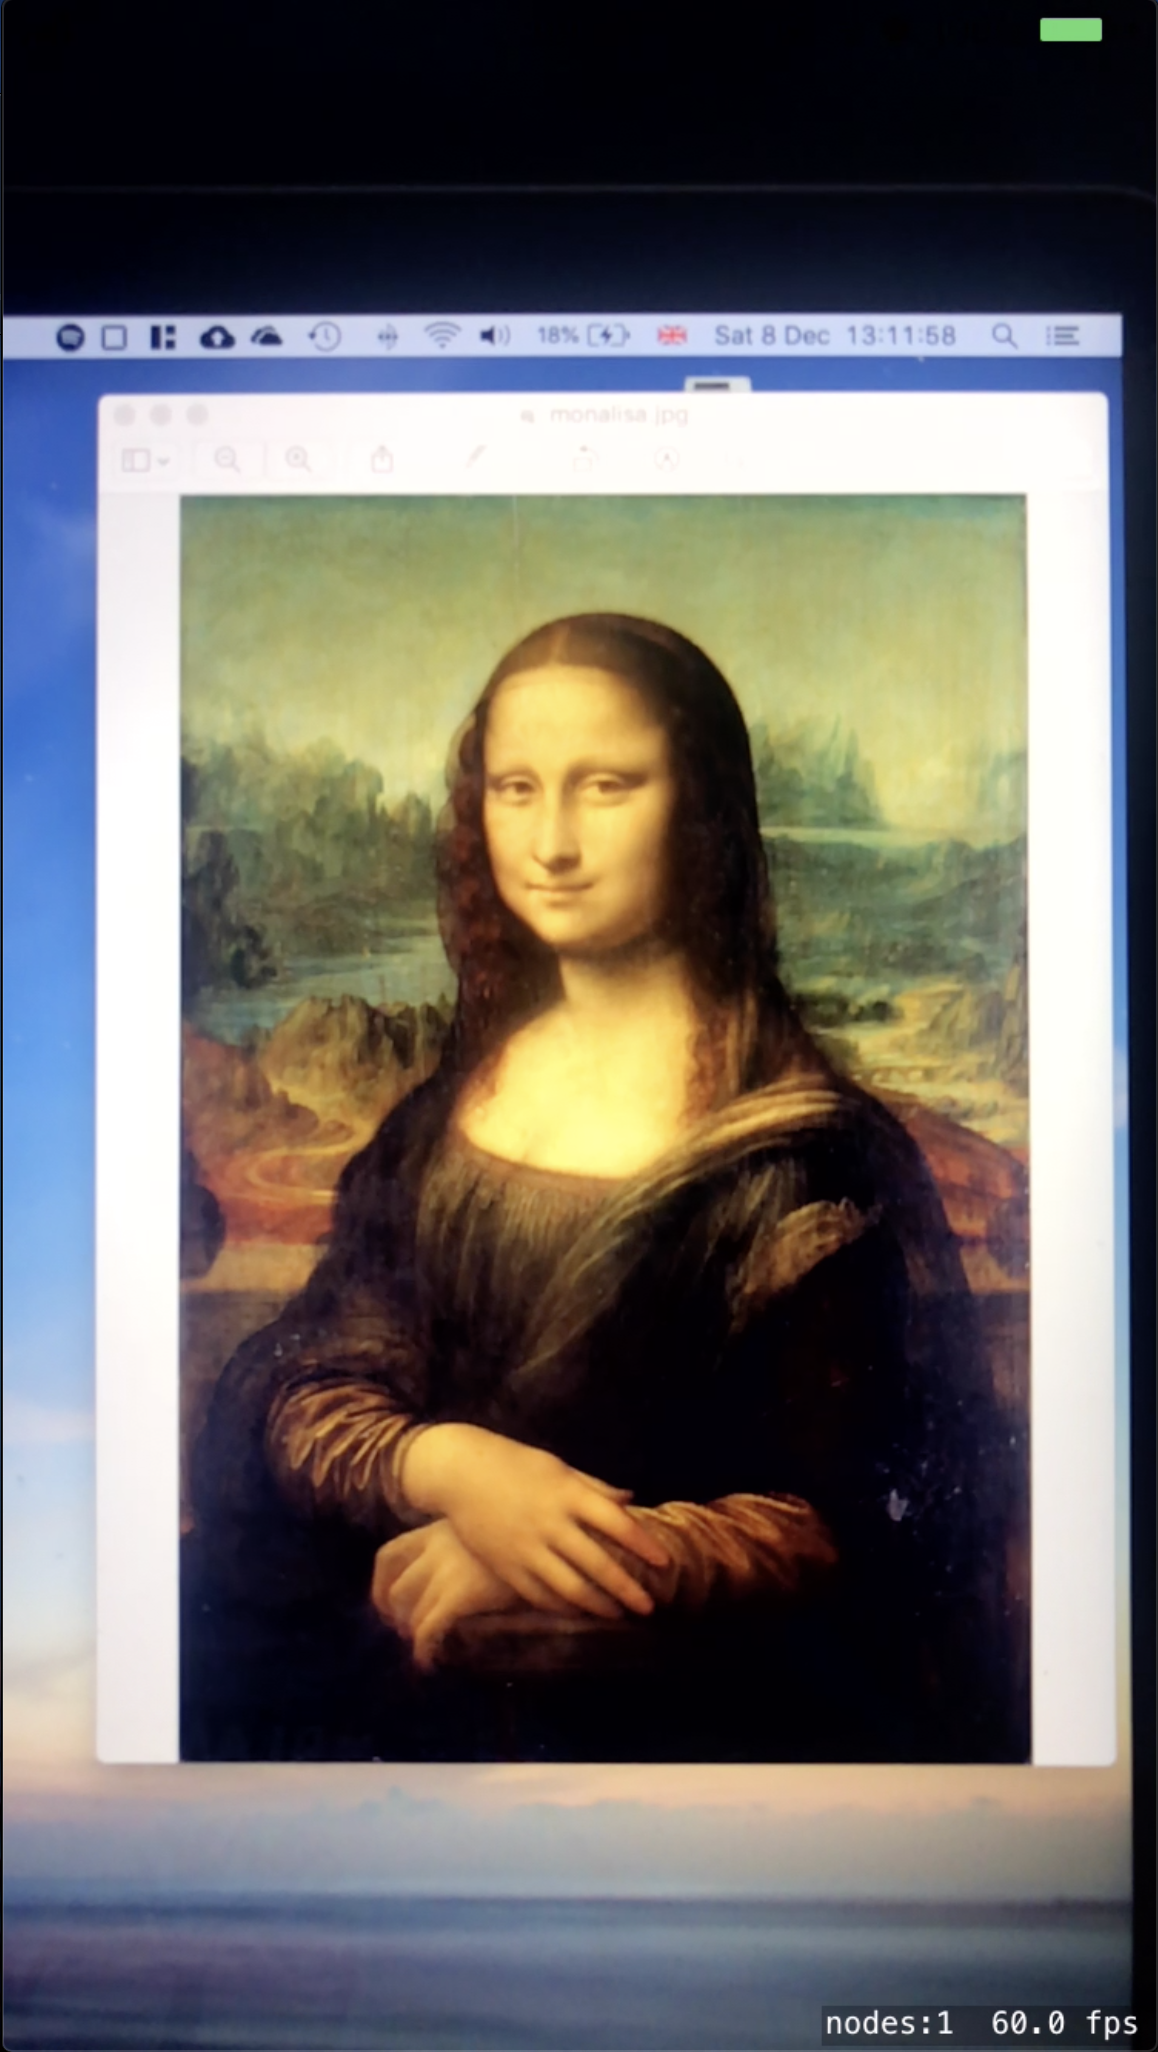
\includegraphics[width=60mm, height=100mm]{prototypes/ar/ios/1.png} &   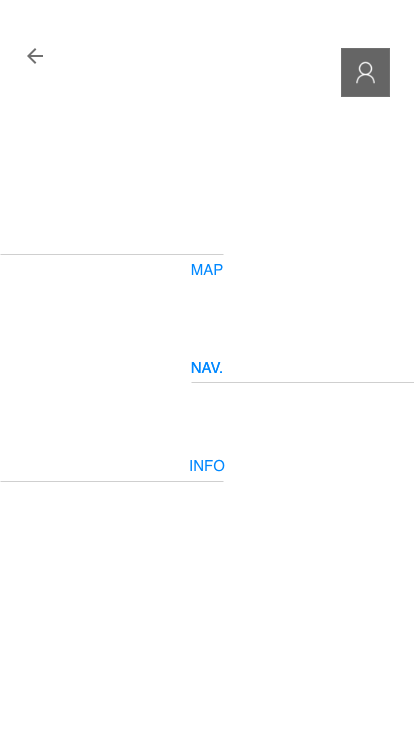
\includegraphics[width=60mm, height=100mm]{prototypes/ar/ios/2.png} \\
% 	(a) Camera over image & (b) Image recognised and displaying information \\[6pt]
% 	\multicolumn{2}{c}{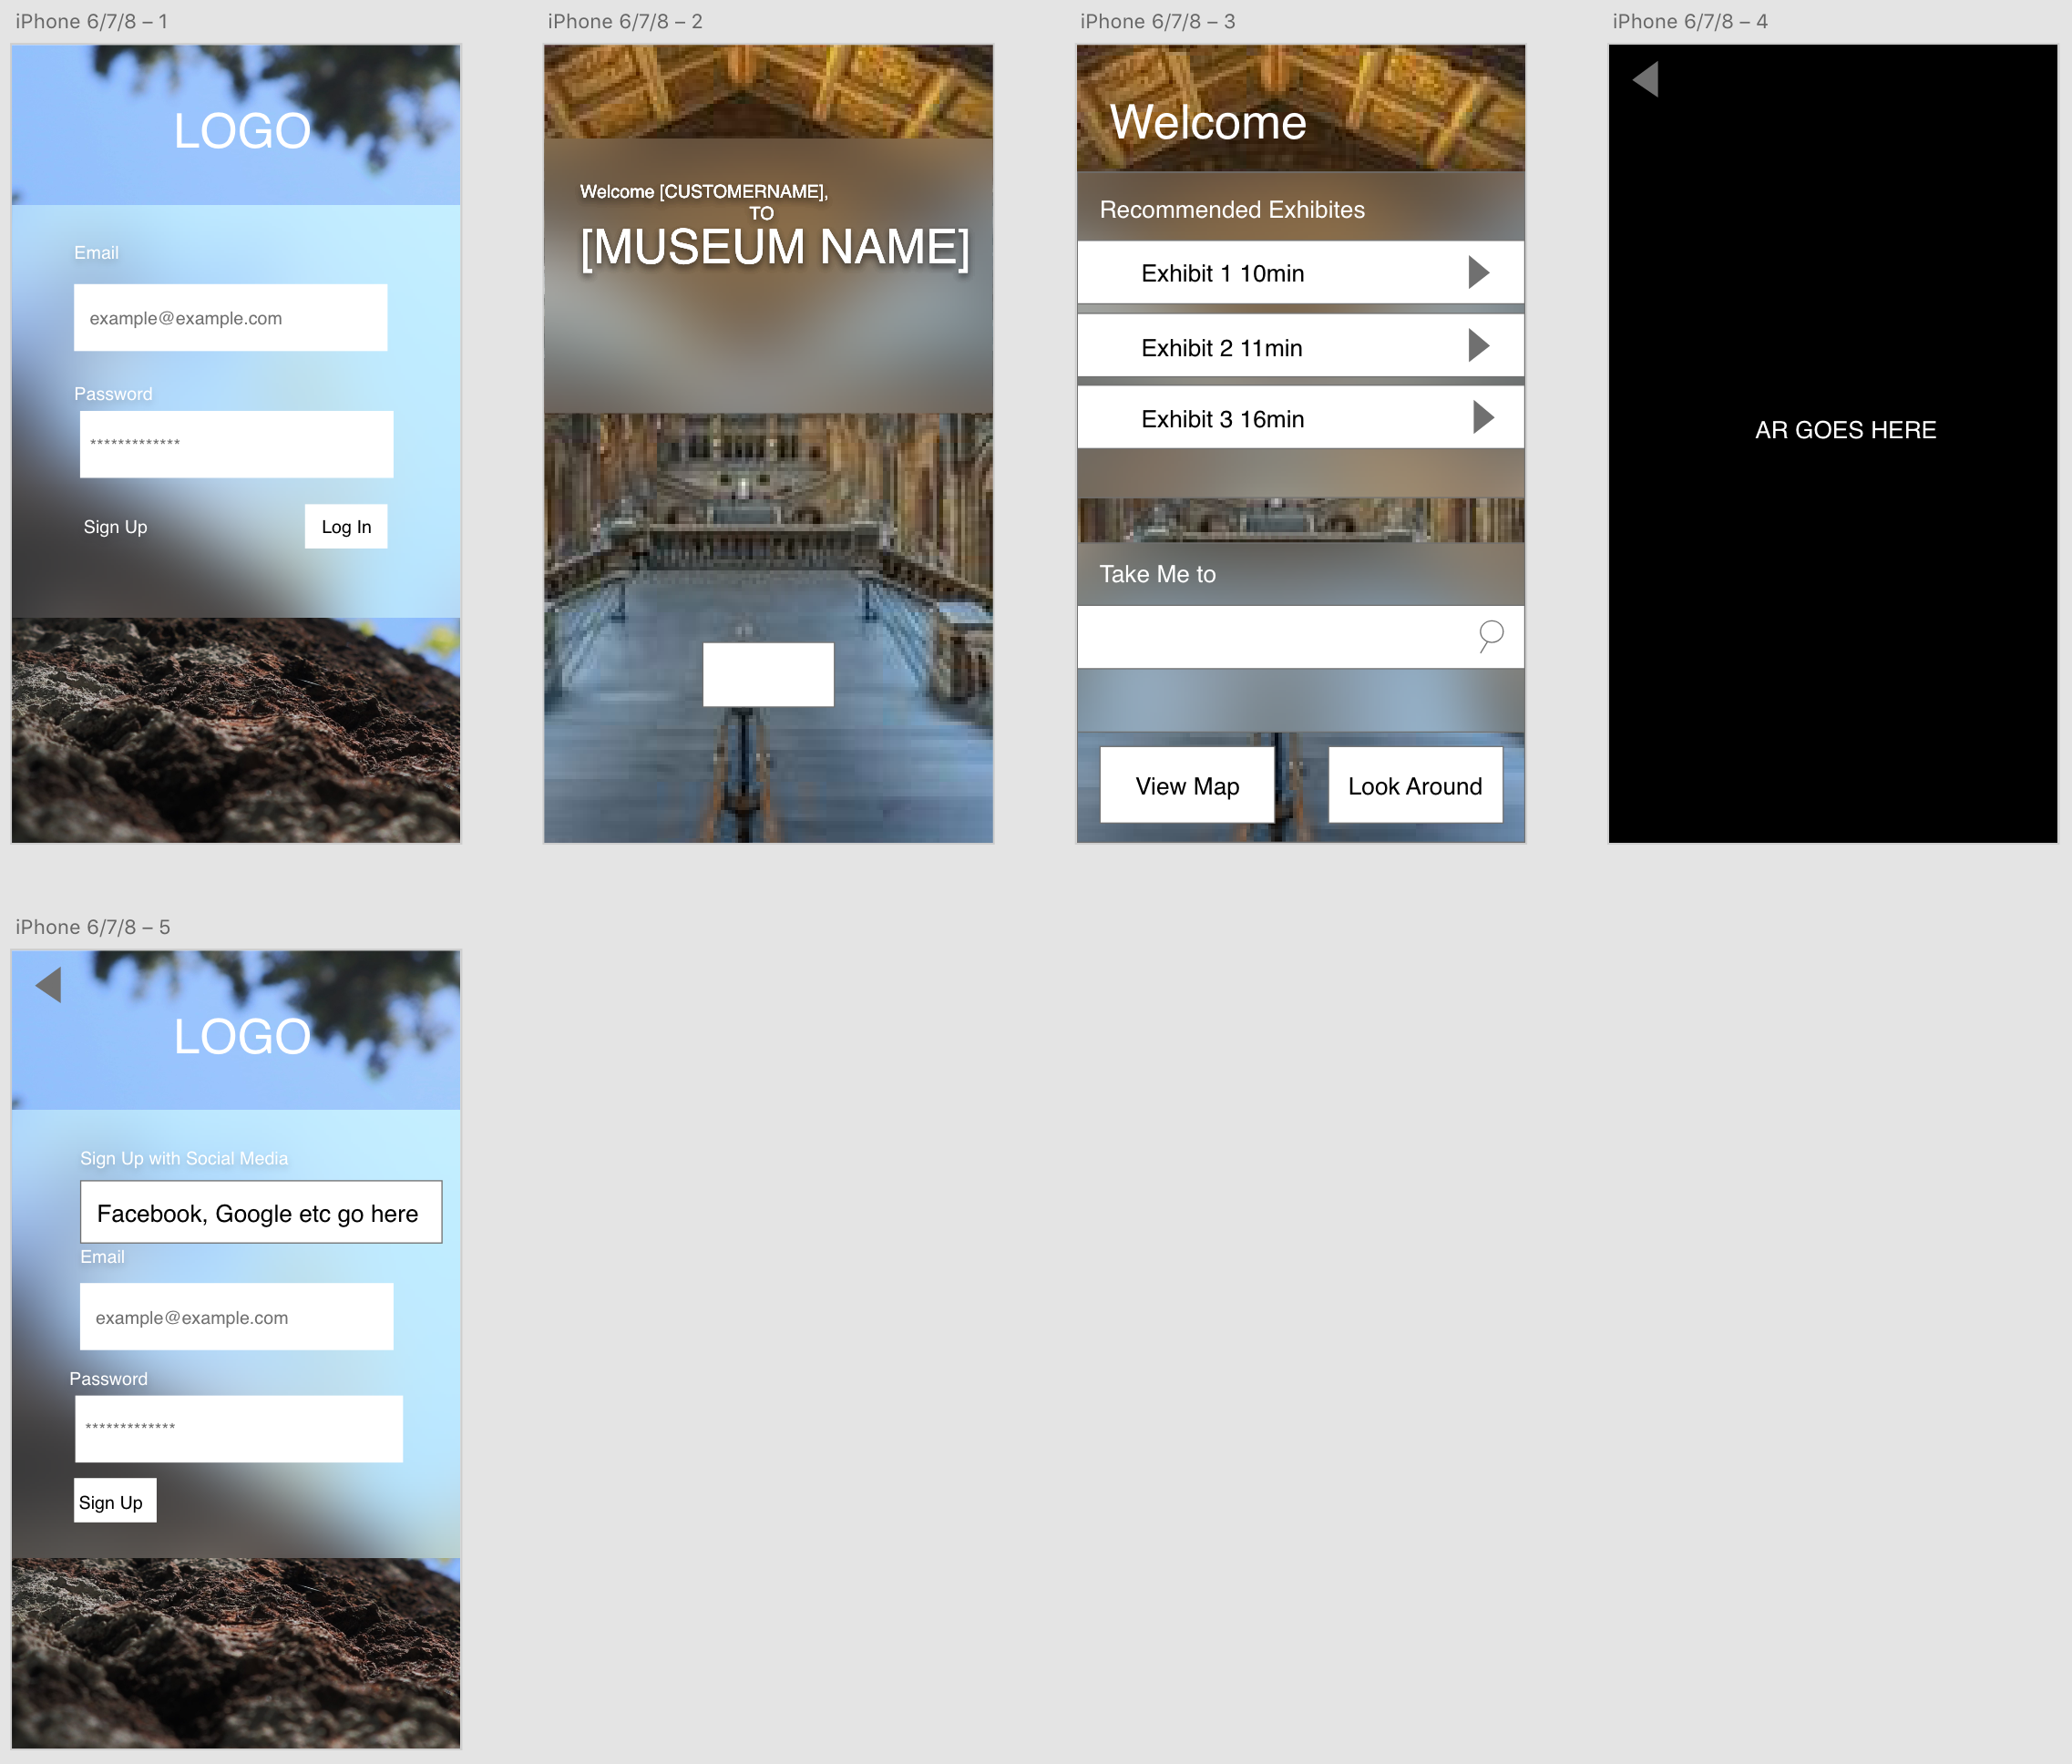
\includegraphics[width=60mm, height=100mm]{prototypes/ar/ios/3.png} }\\
% 	\multicolumn{2}{c}{(c) Image scanned before; showing the green tick}
% 	\end{tabular}
% 	\caption{ARKit prototyping on iOS device}
% 	\label{fig:arlibrary1}
% \end{figure}

\subsection{Vuforia}
Unity is a cross-platform game engine, used to test a simple AR camera prototype where the device’s camera hovers an image, and displays information about that image on the device. The application was built using Vuforia, an SDK that enables recognition, and tracking of image targets. This library can be used for the exploration case in the use case model. Although, there \change{is}{are} a lack of tools for locating user current location compared to Android.

The \change{vuforia}{Vuforia} library was used to test a simple AR camera prototype where the device’s camera hovers an image, and displays information about that image on the device.

Figure here
% \begin{figure}[H]
% 	\centering  
% 	\begin{tabular}{cc}
% 	  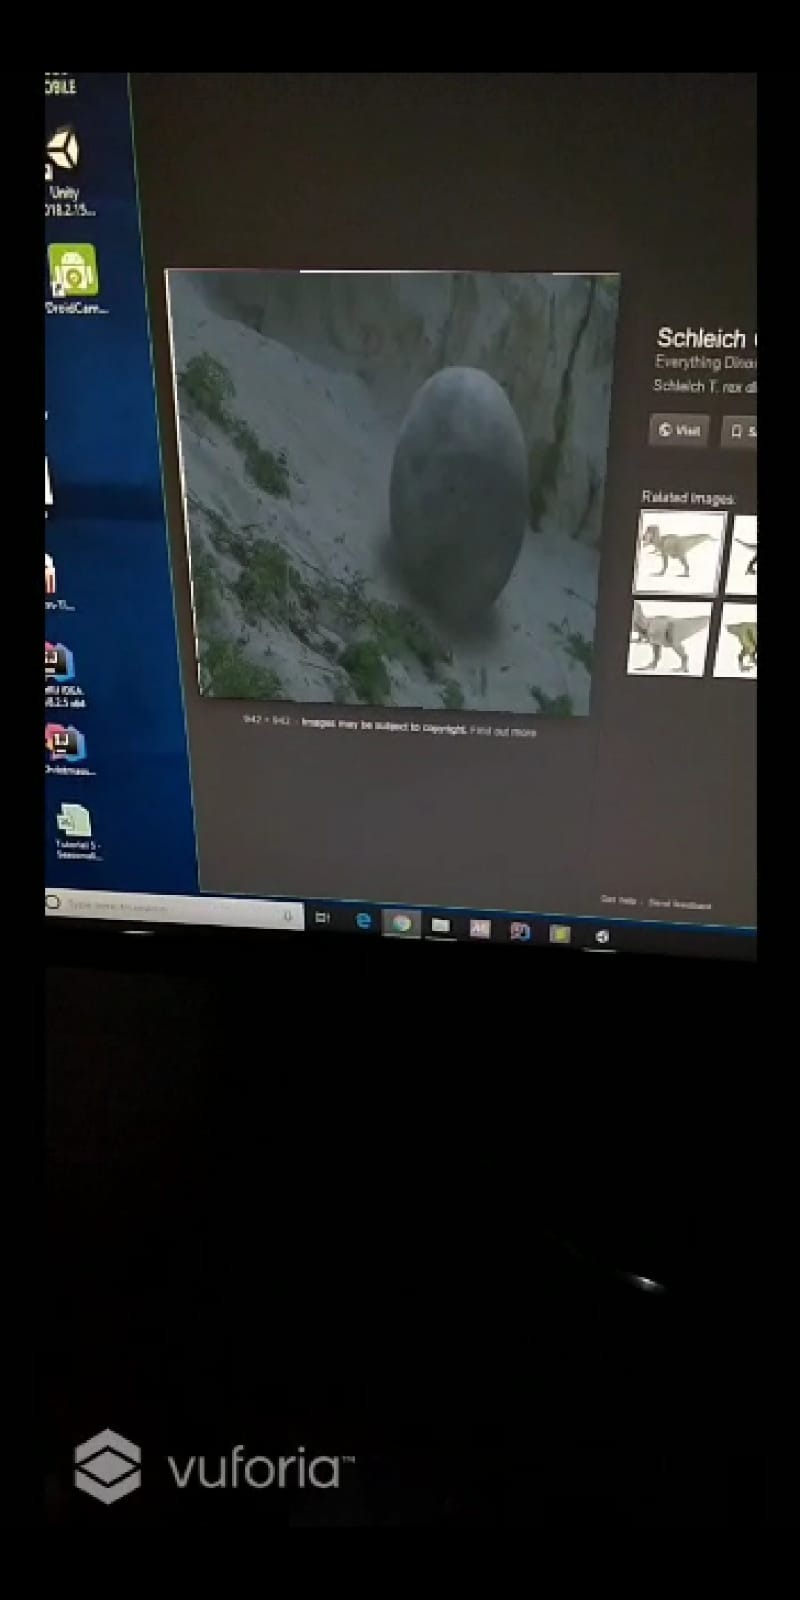
\includegraphics[width=60mm, height=100mm]{prototypes/ar/vulforia/1.jpeg} &   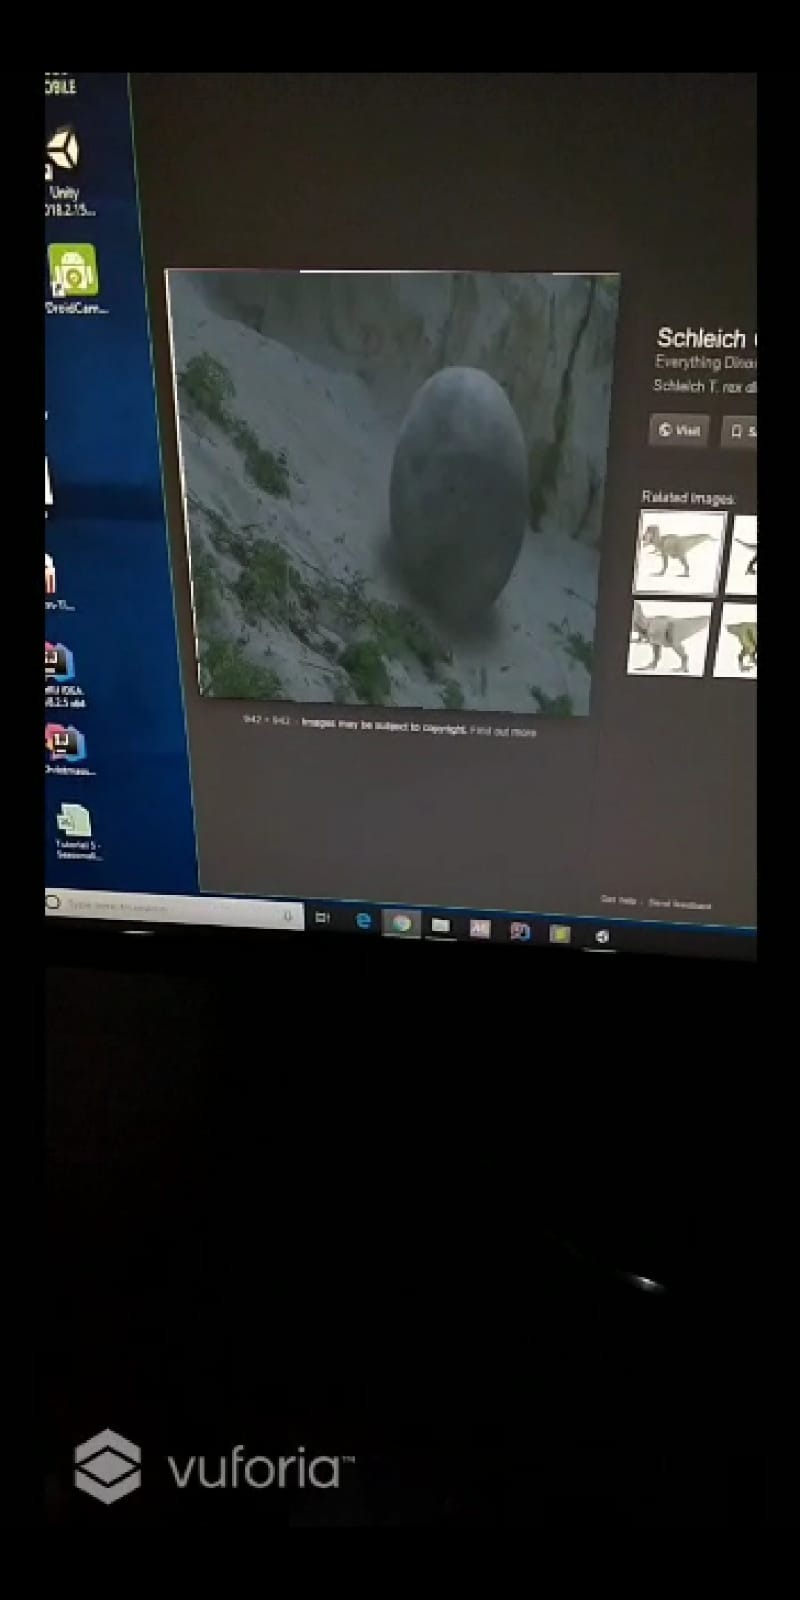
\includegraphics[width=60mm, height=100mm]{prototypes/ar/vulforia/2.jpeg} \\
% 	(a) Camera over image & (b) Video superimposed on top of image\\[6pt]
% 	\end{tabular}
% 	\caption{Vuforia prototyping on Android device}
% 	\label{fig:arlibrary2}
% \end{figure}

\subsection{AR Core (Android)}
AR Core was used to create an AR experience (Figure~\ref{fig:arlibrary3}) giving the user the ability to superimpose a 3D object when the camera is focused on a flat surface.

During the process it was found that \remove{AR Core has noticable differences from the other two libraries. The first difference is that,} unlike ARKit, the library is suitable with Java/Kotlin \change{. Meaning that}{hence} the group would have an easier time acclimating \remove{to} the nature of AR Core. \change{Also because}{As} AR Core is a native Android SDK, it can be integrated with other \remove{natively} android features such as Android's GPS and Android's \change{wifi}{WiFi} libraries. \remove{It's also easier to log data using the AR Core because of how well it has been integrated with the java ecosystem.} \change{One bad difference though is how scattered and vague the documentation is}{Despite this, the documentation was scattered and vageu}, making it a difficult program to debug with. \remove{However, in the end, after}{After} exploring this prototyping process and discussing the accessibility of AR Core(Android) and android to the stakeholders, the group distinguished it as the most suitable library \change{moving forward, regardless}{for the project}. 

Figure here
% \begin{figure}[H]
% 	\centering  
% 	\begin{tabular}{cc}
% 	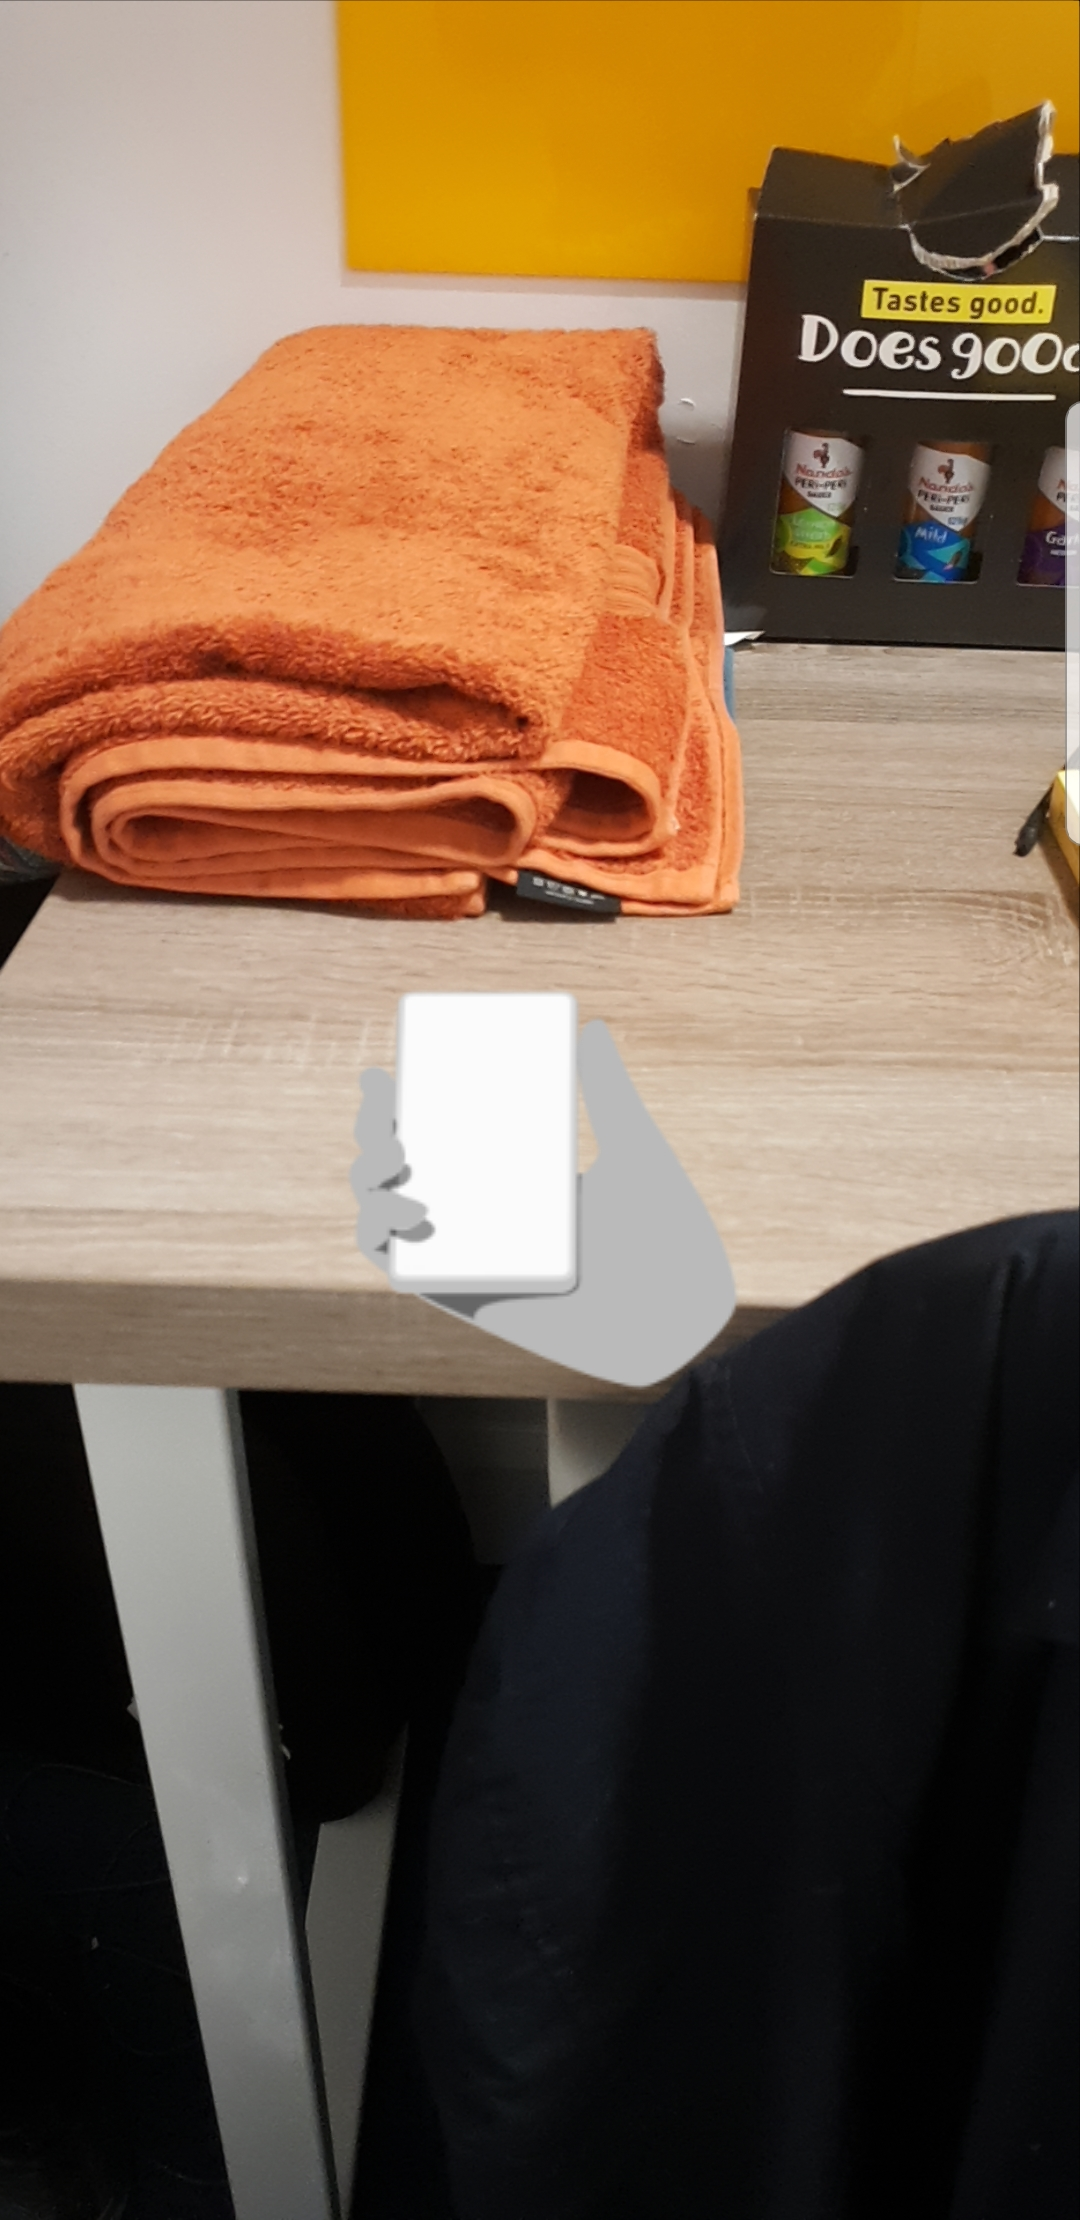
\includegraphics[width=60mm, height=100mm]{prototypes/ar/android/1.jpg} & 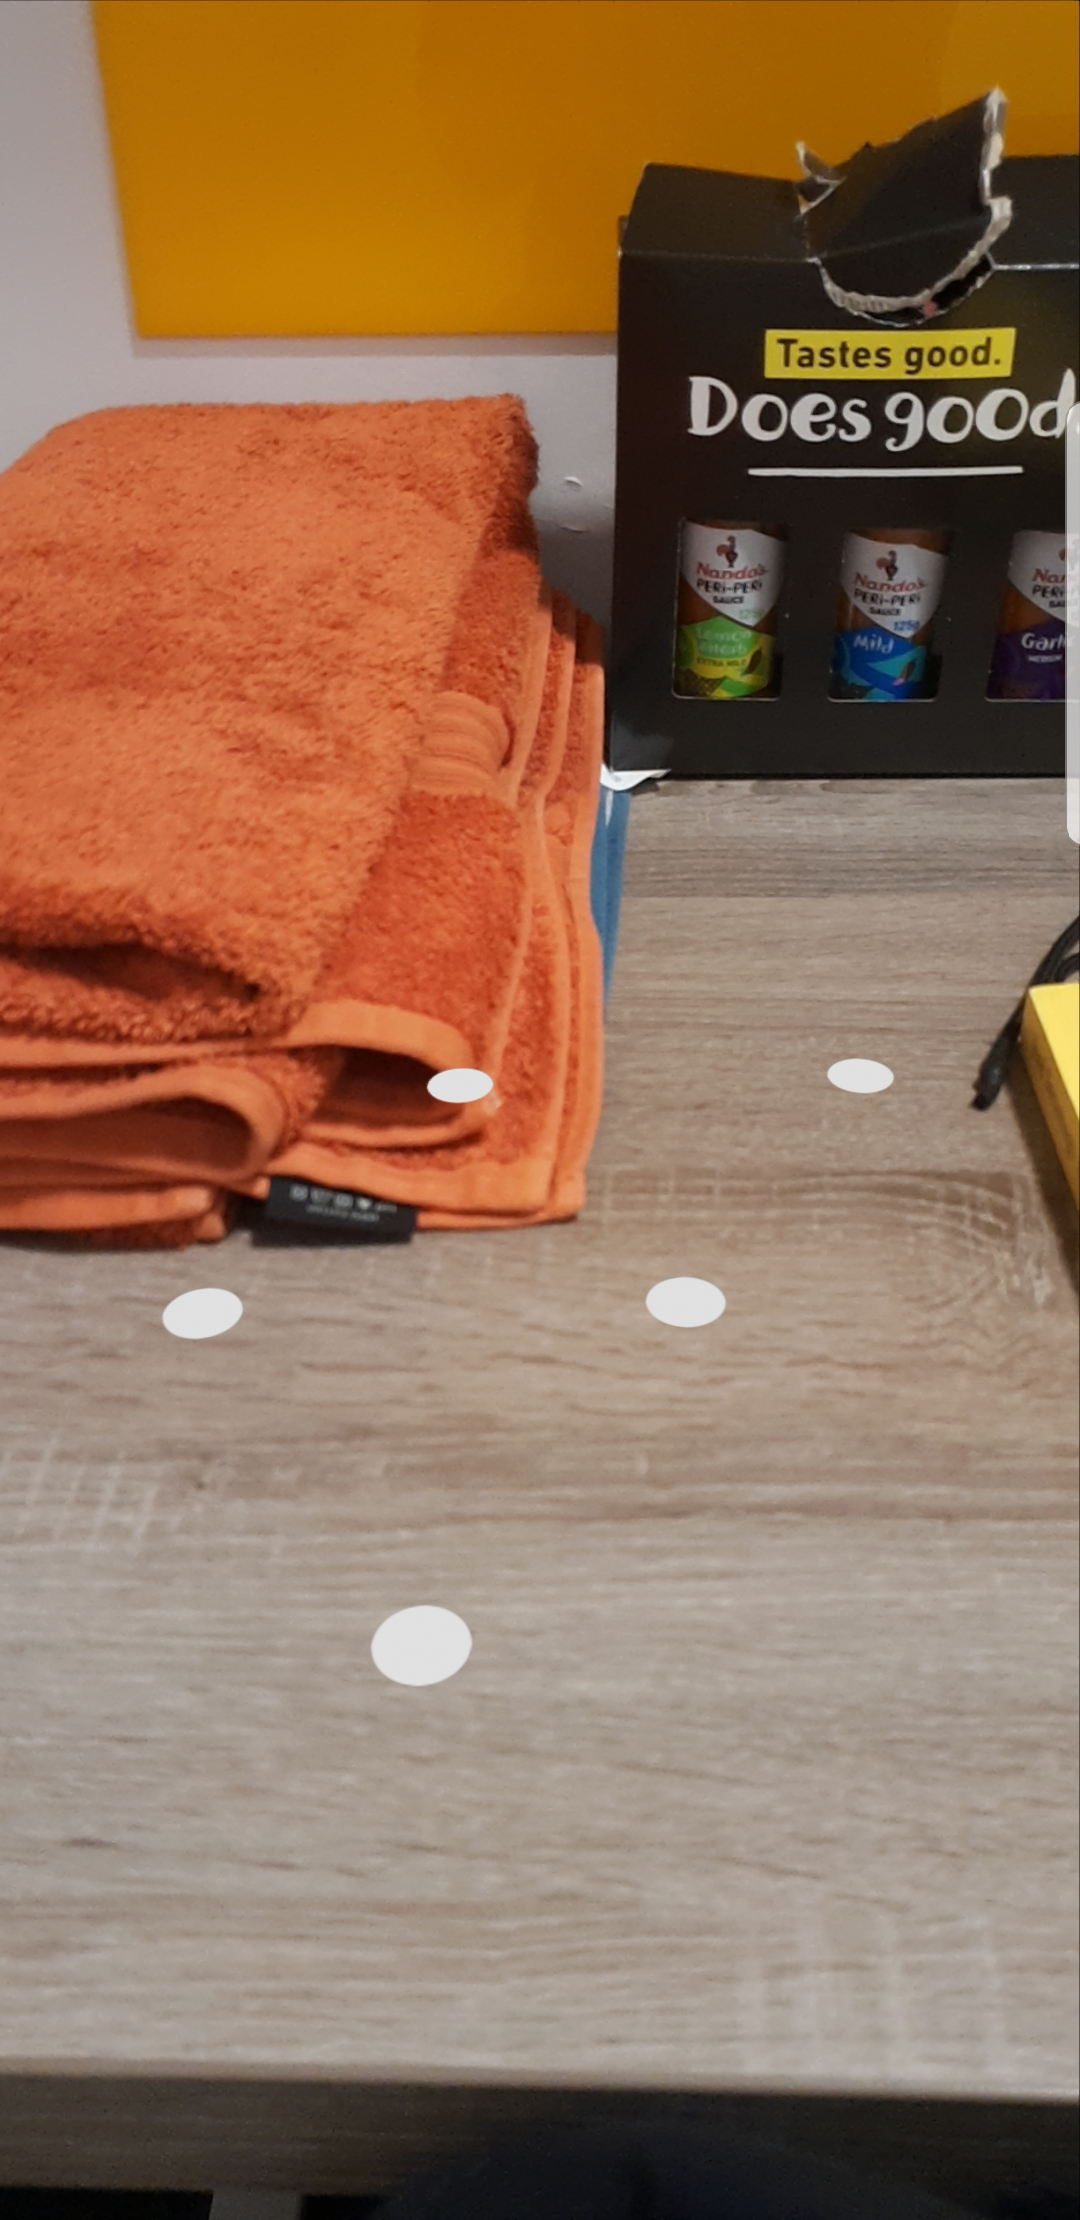
\includegraphics[width=60mm, height=100mm]{prototypes/ar/android/2.jpg} \\
% 	(a) Initial view & (b) Detection of surface \\[6pt]
% 	\multicolumn{2}{c}{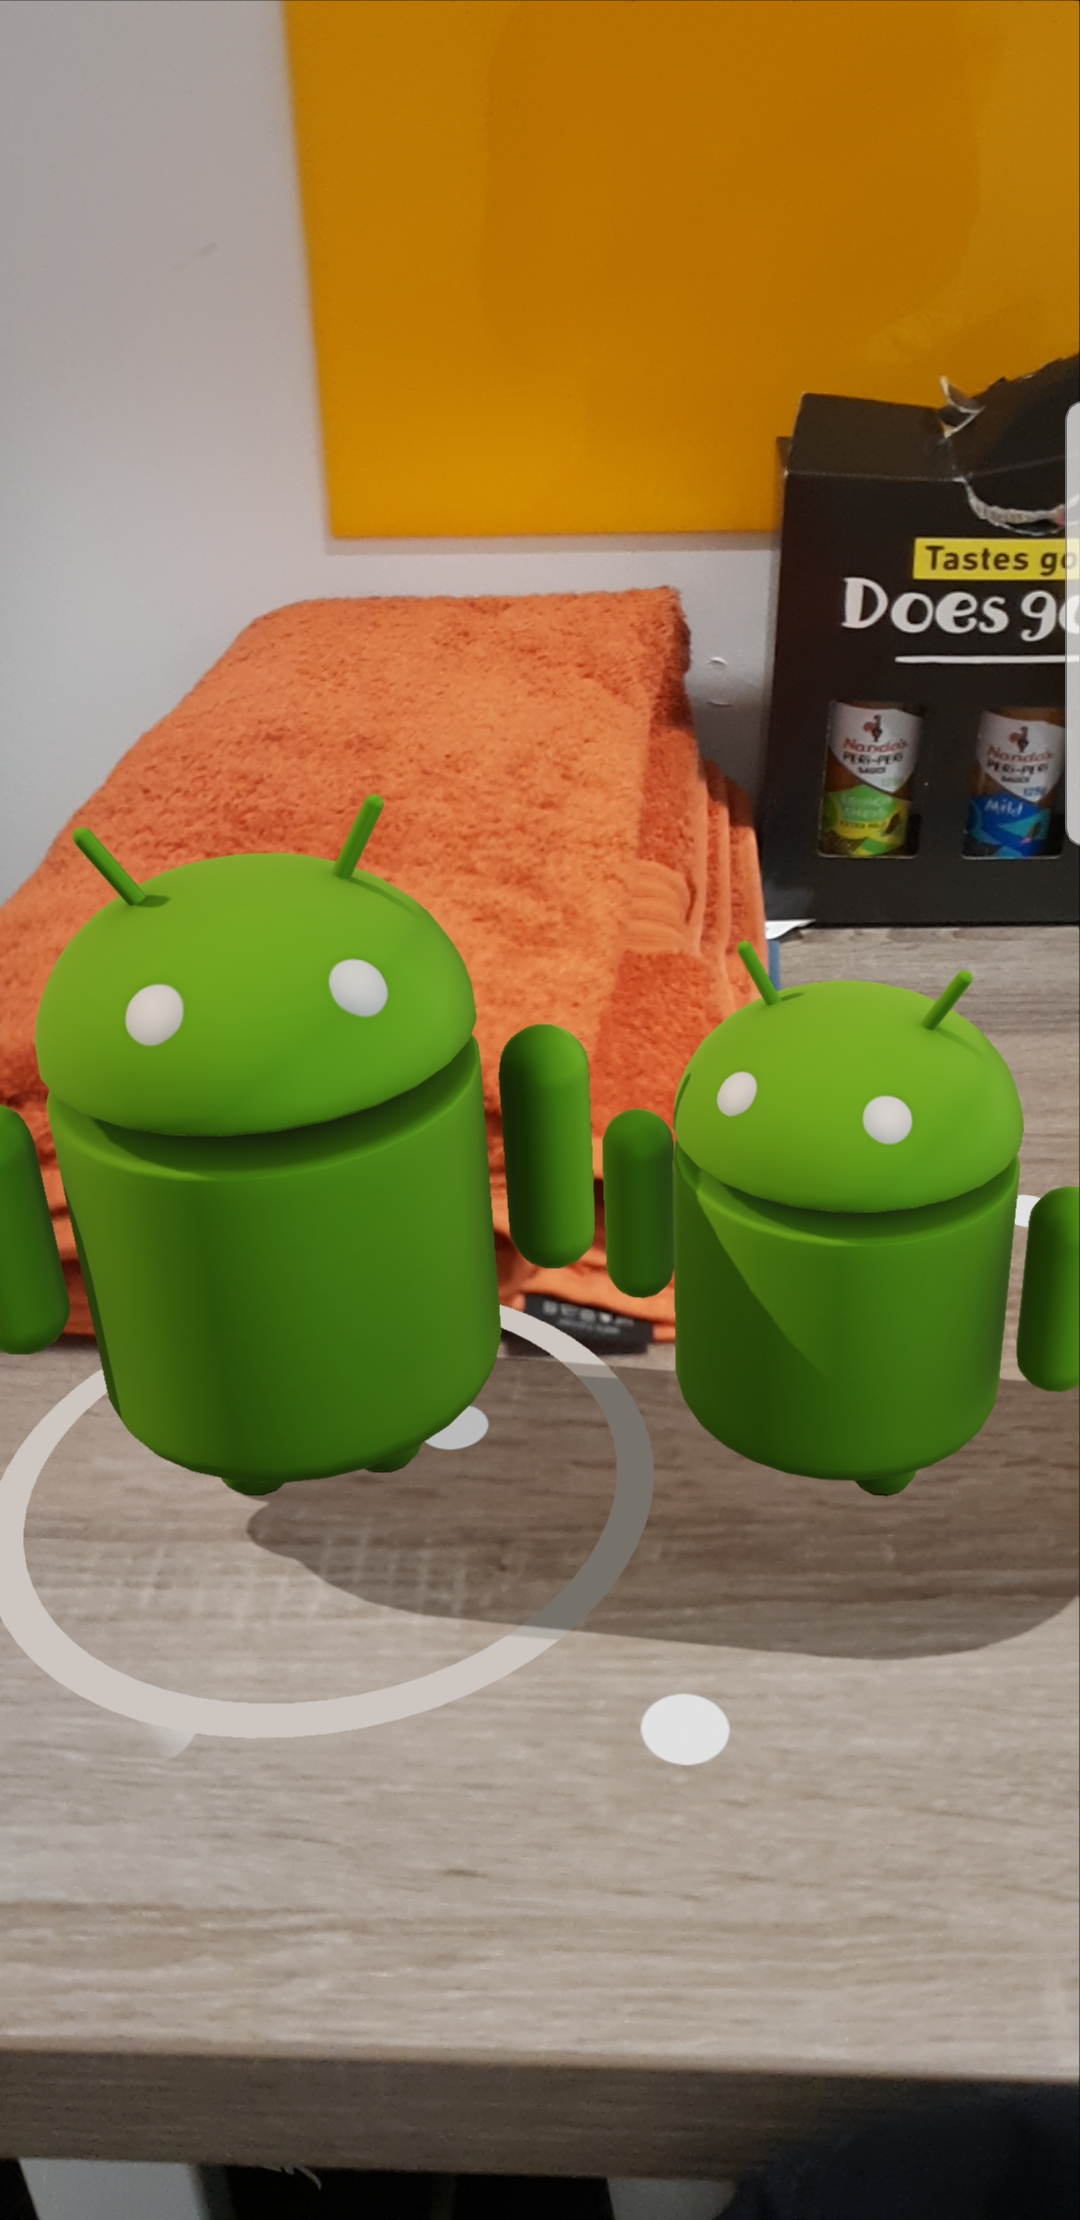
\includegraphics[width=60mm, height=100mm]{prototypes/ar/android/3.jpg} }\\
% 	\multicolumn{2}{c}{(c) Objects superimposed on surface}
% 	\end{tabular}
% 	\caption{ARCore prototyping on Android device}
% 	\label{fig:arlibrary3}
% \end{figure}

\section{Software Architecture}
Hardik Week 1

\annote{A application or computing system's software architecture is a representation of the system that helps to know how the system will operate. By analyzing the current solution on various platforms and devices such as Android and Apple. This will show how we ended up using Android for our application?}{Say why we analysed software architectures}

\annote{We}{no first person} have two various platforms to choose from, as exemplified \annote{in the list}{Wasn't a fan of the bullet points since it's not very common in academic writing} below:
\begin{itemize}
  \item Android
  \item Apple
\end{itemize}

\note{again not a fan of these bullet point, it's better to write in prose so the ideas that you're conveying are more coherent.}
\subsection{Android}
\change{It is an open source operating system developed by Google. It provides SDK for development of application.}{An open-source OS developed by GOogle, it provides an SDK for development of an application.} It \change{use}{uses} \textbf{.apk} extension \change{which}{that} can be downloaded and installed on mobile phones. In order to make AR application, we use ARCore to create our app. There are many advantages and disadvantages when choosing the ARCore for android.
\subsection{Advantages}
\begin{itemize}
  \item Android Emulator - It is nearly three faster in CPU, I/O and RAM compared to ARKit(Apple). This will help our application to load/get faster in user screen. 
  \item Easy to log GPS location compared to iOS.
  \item Easy to build UI with Layout Editor.
  \item Easy to run on multiple android devices such as Samsung, Google Pixel, OnePlus,etc.
  \item Easy to create a simple 3D model that will show on a mobile device when its camera targeted flat surface.
  \item ARCore can detect horizontal surfaces that is similar to motion tracking, and can accurately anchor virtual objects.
  \item Cost effective
\end{itemize}

\subsection{Disadvantages}
\begin{itemize}
    \item It's more difficult to code complex layouts and animations.
\end{itemize}

\subsection{Apple(iOS)}
It is a mobile operating system developed by apple. It provides ARKit SDK for development of application. In order to create an Ar application, you have to use ARKit. There are many advantages and disadvantages when choosing the ARKit for apple.

\subsection{Advantages}
\begin{itemize}
    \item ARKit using the Swift, which is easy to learn.
    \item Stable and fast motion tracking.
    \item It helps to load our application in user screen faster.
\end{itemize}

\subsection{Disadvantages}
\begin{itemize}
    \item limitation of ARKit map compare to Android
    \item Not easy to log GPS location.
    \item It is not flexible only support iOS devices.
    \item Not easy to create an 3D model for naviagation.
\end{itemize}


\section{Hardware - Arduino and Raspberry Pis}
Nick Week 1
% changes fixed
As part of our exploration it was recommended, based off lengthy research and from an interlocution with the project’s domain expert the need for a to a physical beacon. 

This role of this beacon, no matter the configuration, was to broadcast a signal. Three main current technologies exist exist: optical infra-red, Bluetooth and, WiFi. Speaking to industry specialists, the former – which underpins their navigation technology and would yield pin-point accuracy – important if you are dealing with small indoor spaces, but this is expensive; Bluetooth, while less accurate, is far cheaper to manufacture and develop; the latter-most (thricely), WiFi offers the least in accuracy and not too expensive. From this probing, Bluetooth became the team’s solution.

Turning in to more a physical project which was not anticipated, a task was set to design a beacon. Looking at relatable past projects, the favourable direction was using a Arduino (UNO R3 Mega 2560) or the Raspberry Pi 3 Model B+. Both solutions gave a clear, small and light-weight canvas on which to design our beacon. However, with a smaller physical footprint – also in keeping with the project’s eco-friendly policy, the Arduino was cheaper. This was a priority to get the technology to have a wide-spread appeal. 

Taking forward the Arduino platform, it was kitted out with a Bluetooth HC-05 RF transceiver. This setup was able to broadcast a simple Bluetooth signal where software can decipher a signal strength from which a distance could be determined. Despite this, it became apparent that there was a need to have further invest in more beacons to give a more accurate and reliable result via triangulation. This was not a suitable solution as one underpinning goal of this project is to make our technology assessable and available to a wide range of applications – an increase in cost would hinder this.

\note{can we add some photos of the arduino we used?}